\documentclass[12pt]{article}

\usepackage{amsmath}
\usepackage{amssymb}
\usepackage{amsfonts}
\usepackage[style=iso]{datetime2}
\usepackage[explicit]{titlesec}
\usepackage{amsthm}
\usepackage{array}
\usepackage{graphicx}
\usepackage{float}

\graphicspath{ {./Images/} }

\theoremstyle{definition}
\newtheorem{problem}{Problem}
\newtheorem{definition}{Definition}

\begin{titlepage}
\title{Calculus I: Introduction to Limits}
\author{The Melon Man}
\date{\today}
\end{titlepage}

\renewcommand{\thesection}{\Roman{section}}

\allowdisplaybreaks

\setlength{\parindent}{0pt}
\setlength{\parskip}{1em}

\begin{document}
\maketitle

In the previous section, we looked at different problems where we wanted to know the behaviour of some function around a point $x=a$.
We no longer care about where our functions are gotten from as we just want to analyse the functions themselves.
In all of the questions in the last section, we chose values of $x$ getting closer and closer to our target value $x=a$ (from both sides) until we could estimate the value at that point.

This process is called taking the limit, and there is notation for it.
The notation for the two main problems in the previous section is shown below.

\begin{equation*}
    \lim_{x\to1} \frac{-2x^2+2}{x-1} = -4 \qquad \lim_{t\to5} \frac{t^3-6t^2+25}{t-5} = 15
\end{equation*}

This notation has us sepcifying the function we are taking the limit of and the value which our variable approaches.
Instead of looking at the actual methods to compute limits, we will look at the intuition behind them to see what they actually represent.
The methods of estimating limits that will be used are not typically used to actually compute them; it may be quite difficult to estimate the value of the limit or it may sometimes give the wrong value.
Actually computing limits will be discussed in later section.
Below is a 'definition' of a limit.

\begin{definition}
    The limit of $f(x)$ is $L$ as $x$ approaches $a$, written as

    \begin{equation*}
        \lim_{x\to a} f(x) = L, \label{eq:1}
    \end{equation*}

    if $f(x)$ can be made to be close to $L$ for all values of $x$ close to $a$, from both sides, with $x\neq a$.
\end{definition}

Now this is not a precise, formal definition of a limit.
That will be covered in a later section.
The above definition gives an idea of how a limit works and what it tells us about functions.
Suppose we know a limit does exist.
According to our definition, we can choose how close $L$ will be to $f(x)$.
Say we want the difference between them to be no more than $0.001$, we want one of the following.

\begin{align*}
    f(x) - L & < 0.001 \qquad \text{if } f(x) \text{ is larger than L}  \\
    L - f(x) & < 0.001 \qquad \text{if } f(x) \text{ is smaller than L}
\end{align*}

If the limit does exist, then we can get $x$ close enough to $a$ to make either of the above statements true.
Precisely, our definition states that there is some value of $x$, say $X$, such that for all $x$ closer to $a$ than $X$, one of the statements will be true.
The idea that the difference between $f(x)$ and $L$ must stay small for all values of $x$ such that the difference between $x$ and $a$ is small is quite important; there are many functions where we can make $f(x)$ close to $L$ for values of $x$ close to $a$ but there are values of $x$ even closer to $a$ that does not make $f(x)$ close to $L$.
Such an example will be discussed later on.
For a limit to exist, $f(x)$ must stay close to $L$ (or get closer) for all values of $x$ that are sufficiently close to $a$.

In simpler terms, as $x$ gets close to $a$, $f(x)$ must get close to $L$.
It is important to note that we must look at values of $x$ close to $a$ from both sides of $x=a$.
Also, the definition excludes $x=a$; while limits are used to discover the behaviour of a function at some point $x=a$, the limit is not concerned with what happens at $x=a$ itself.
Rather, it looks at the behaviour around that point.
This is another important concept to remember.

One alternative notation for the limit of $f(x)$ to $L$ as $x$ approaches $a$ is the following.

\begin{equation}
    f(x) \to L \quad \text{as} \quad x \to a
\end{equation}

To use Definition~\eqref{eq:1} to help estimate limits, we shall use the method we did in the previous section.
We evaluate $f(x)$ for values of $x$ getting closer and closer to $a$ and see if it approaches some value $L$.
Below is an example of this.

\begin{problem}
Estimate the value of:
\begin{equation*}
    \lim_{x \to 2} \frac{x^2+4x-12}{x^2-2x} \label{eq:2}
\end{equation*}
\end{problem}

We will only be estimating the value of this limit and look at actually computing limits later.
This is to show what the limit tells us about the function.
To estimate it, we will pick values of $x$ getting closer and closer to $x=2$ and plug them into our function.
The table of values for this is below.

\begin{table}[h]
    \renewcommand{\arraystretch}{1.5}
    \centering
    \begin{tabular}{>{\centering\arraybackslash}m{1.5cm}|>{\centering\arraybackslash}m{2.5cm}|>{\centering\arraybackslash}m{1.5cm}|>{\centering\arraybackslash}m{2.5cm}}
        $x$       & $f(x)$        & $x$       & $f(x)$        \\ \hline
        $2.5$     & $3.4$         & $1.5$     & $5$           \\
        $2.1$     & $3.857142857$ & $1.9$     & $4.157894737$ \\
        $2.01$    & $3.985074627$ & $1.99$    & $4.015075377$ \\
        $2.001$   & $3.99850075$  & $1.999$   & $4.00150075$  \\
        $2.0001$  & $3.999850007$ & $1.9999$  & $4.000150008$ \\
        $2.00001$ & $3.999985$    & $1.99999$ & $4.000015$
    \end{tabular}
\end{table}

From the table, we can see that $f(x)$ approaches 4 as our $x$ values approach $x=2$ from both sides (using $x$ values very close to $x=2$ to ensure as much accuracy as possible with our estimation).
Therefore, we can estimate that our limit, the answer to Problem~\eqref{eq:2}, evaluates to 4.
We may not be able to evaluate the function at $x=2$, as that would lead to us dividing by 0, but this does not matter; our limit is only concerned with what happens as we go to $x=2$ and not directly at $x=2$.
It turns out to be the case that this is the actual value of limit, which we will cover in a later section, so we may write the following.

\begin{equation}
    \lim_{x \to 2} \frac{x^2+4x-12}{x^2-2x} = 4
\end{equation}

To get a better idea of what this limit shows us, it would be a good idea to graph the function in Problem~\eqref{eq:2} in the range of $x$ values we care about.
That is shown below.

\begin{figure}[H]
    \centering
    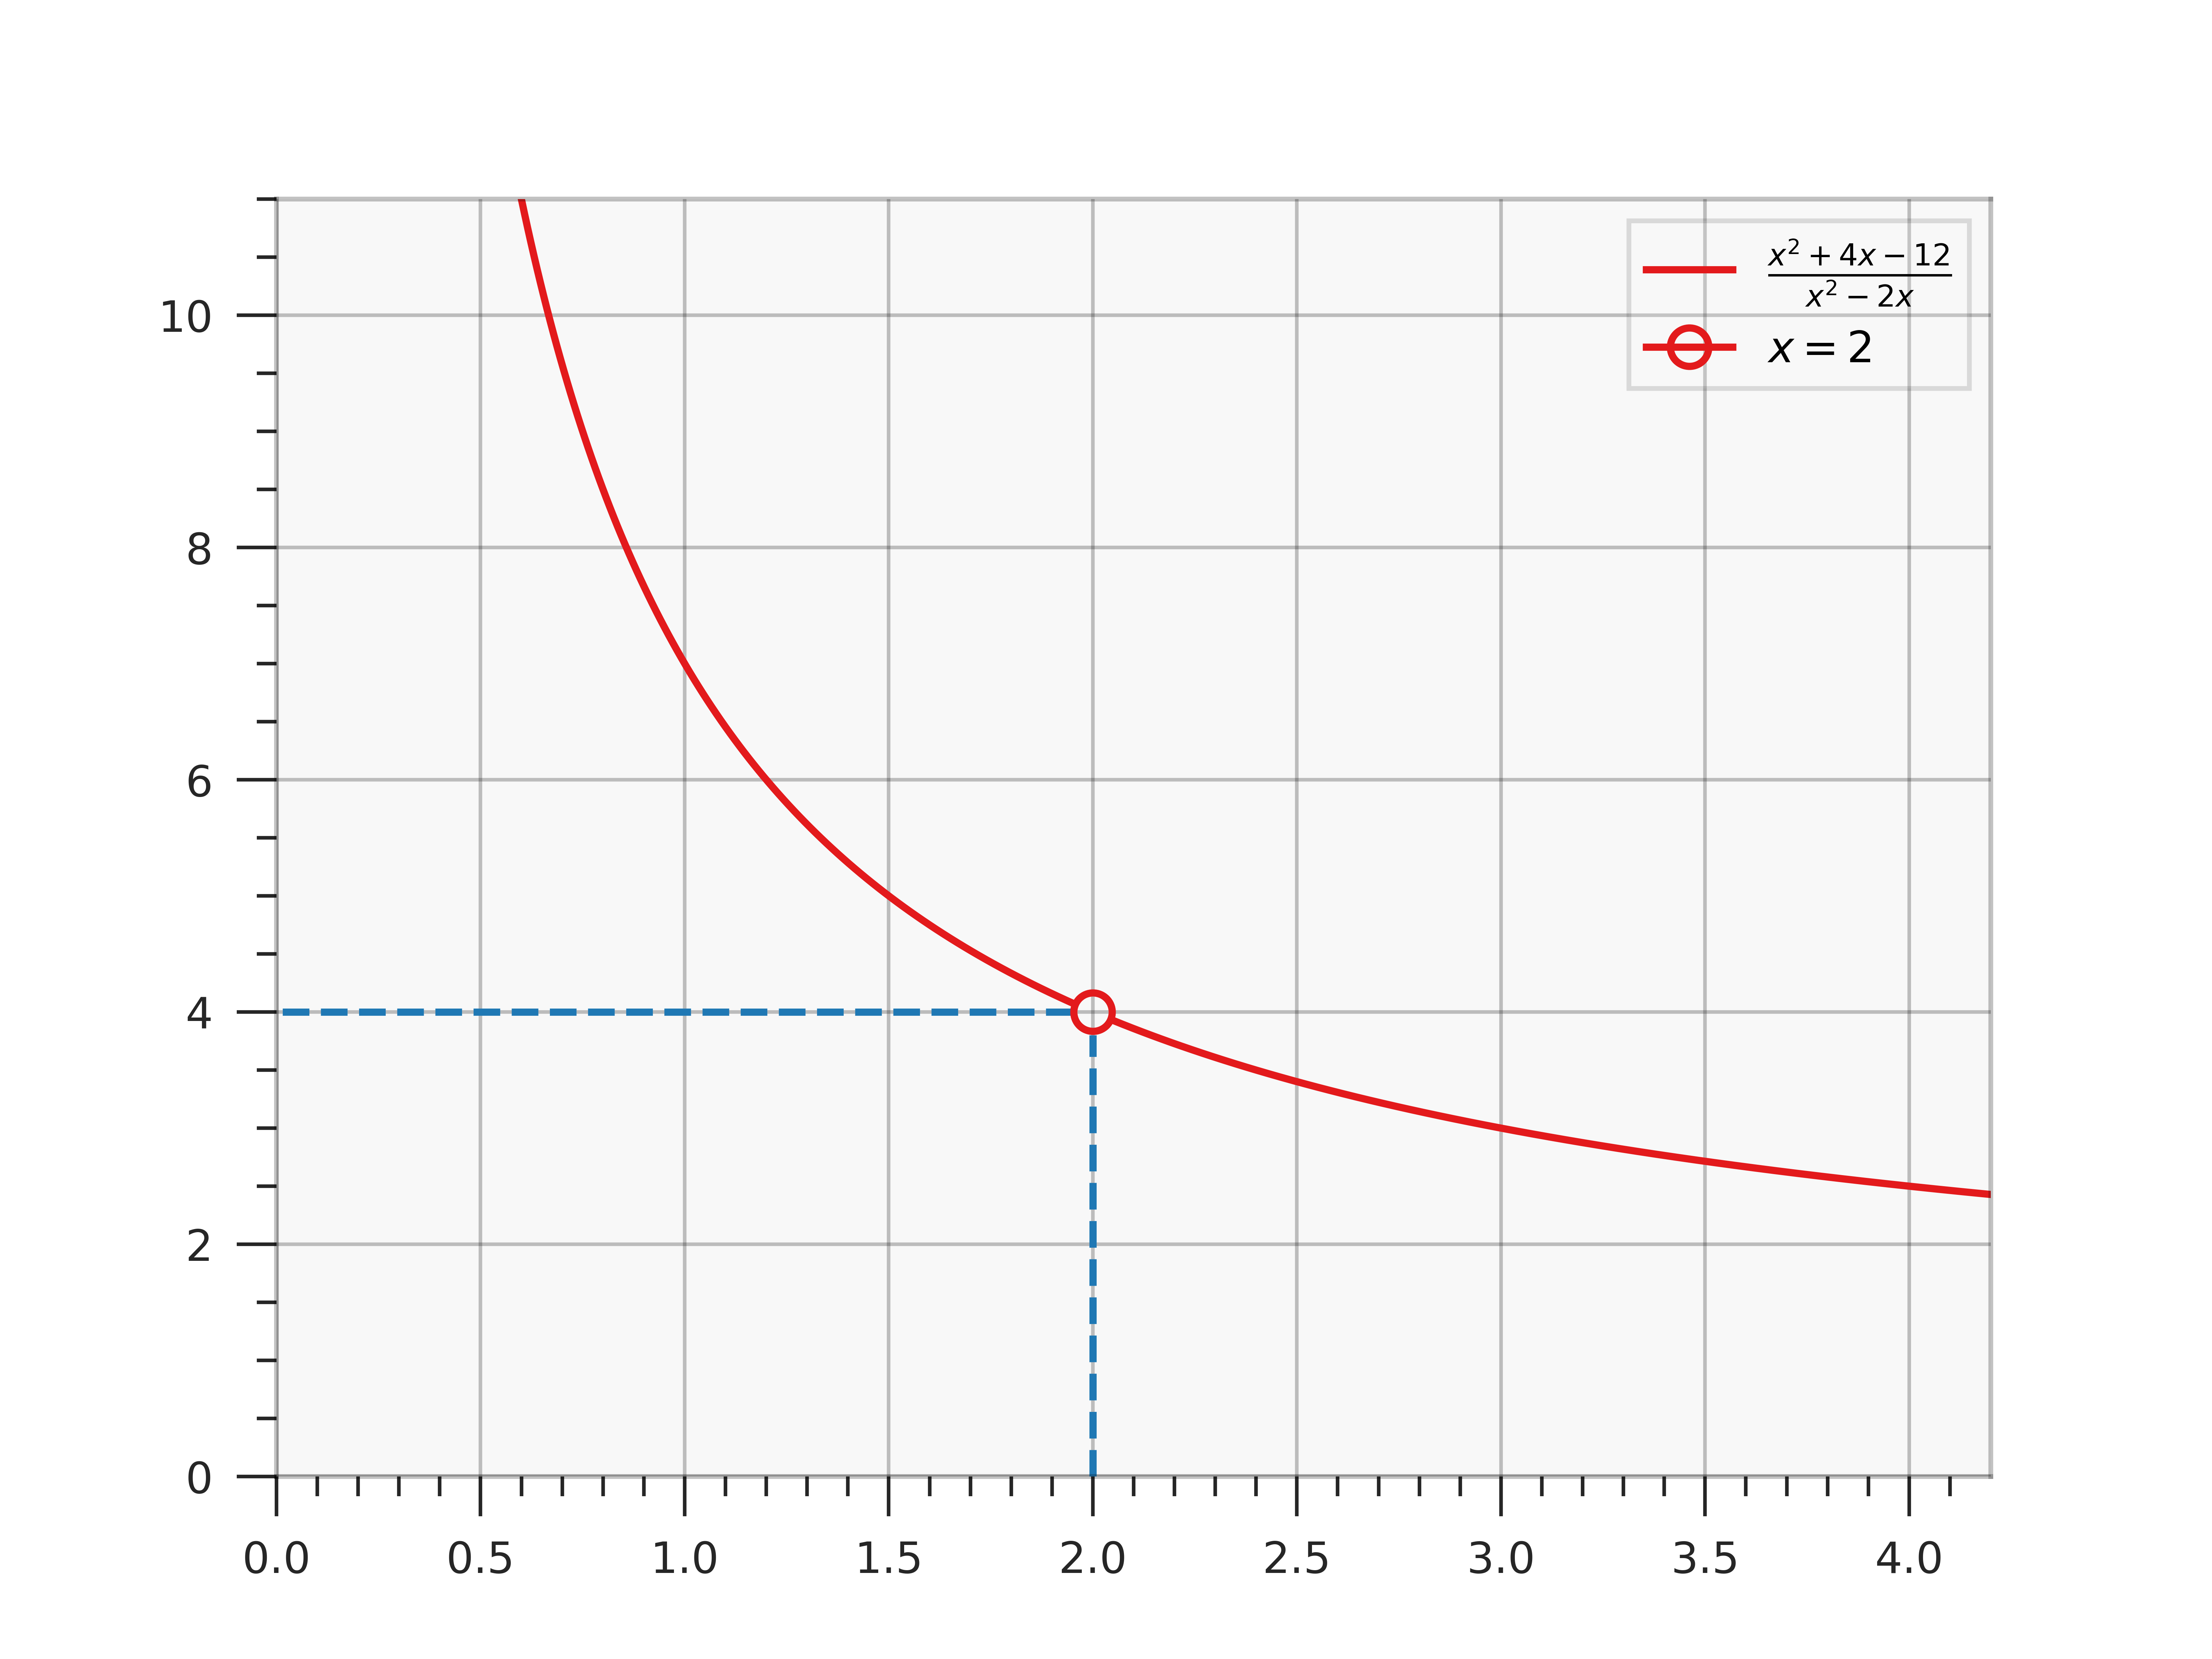
\includegraphics[width=12.5cm, keepaspectratio]{limits_1.png}
    \caption{Limits}
    \label{fig:fig1}
\end{figure}

Note that the large open dot on the graph at $x=2$ is to show that the function does not exist at $x=2$ (division by 0).
As we plug values of $x$ into our function, we are moving along the graph towards $x=2$; using values both larger and smaller than 2 shows us approaching the point from both the right and left respectfully.
When computing limits, we do not care what the value of a function is at our target value, if any.
Here, while the function does not exist at $x=2$, the limit certainly does as we can clearly see from the graph that $f(x)$ approaches 4 as $x$ approaches 2, from both sides.
Therefore, the limit is 4.

Overall, the main point that we saw from the previous example is that we do not care about what value a function is at some point when taking its limit.
Instead, we care about what happens around that point and what value it approaches.
Even if a function is not defined at some point, it may have some limit at that point if it approaches some value from both sides of that point.
This is good as many functions have points where they do not exist, but they still approach some value and thus have a limit.
The next example will show this further with a slight variation.

\begin{problem}
Estimate the value of:
\begin{equation*}
    \lim_{x \to 2} g(x), \quad g(x) =
    \begin{cases}
        \frac{x^2+4x-12}{x^2-2x} & \text{if } x \neq 2 \\
        6                        & \text{if } x = 2
    \end{cases} \label{eq:3}
\end{equation*}
\end{problem}

This piecewise function $g(x)$ is exactly the same as the function in Problem~\eqref{eq:2}, except for the fact that it is defined at $x=2$.
Thus, the following is true by way of our function's definition.

\begin{equation*}
    g(2) = 6
\end{equation*}

To estimate the value of our limit, nothing has changed from the previous problem.
If we created a table of values for $g(x)$, it would look exactly like the previous one we did.
We could estimate using a table of values or by looking at the graph of $g(x)$; our result remains the same.

When we had created a table of values for the previous problem, we did not put $x=2$ in the table.
That is because we do not care about its value, or lack theirof in the case of Problem~\eqref{eq:2}.
The value at $x=2$ could not exist, or be a completely different value (such as 6) from what the function actually approaches.
The limit will not change.
Since the table of values would be the same and we already know our estimation for Problem~\eqref{eq:2} is the actual value of the limit, our solution to Problem~\eqref{eq:3} is the following.

\begin{equation}
    \lim_{x\to2} g(x) = 4
\end{equation}

The limit is not 6.
Since the only difference between $g(x)$ and the previous function is its value at $x=2$ itself, the limit is the same; limits do not care about the value at the target point but only the function's behaviour as we approach the point.
This may be illustrated with a graph of $g(x)$.

\begin{figure}[H]
    \centering
    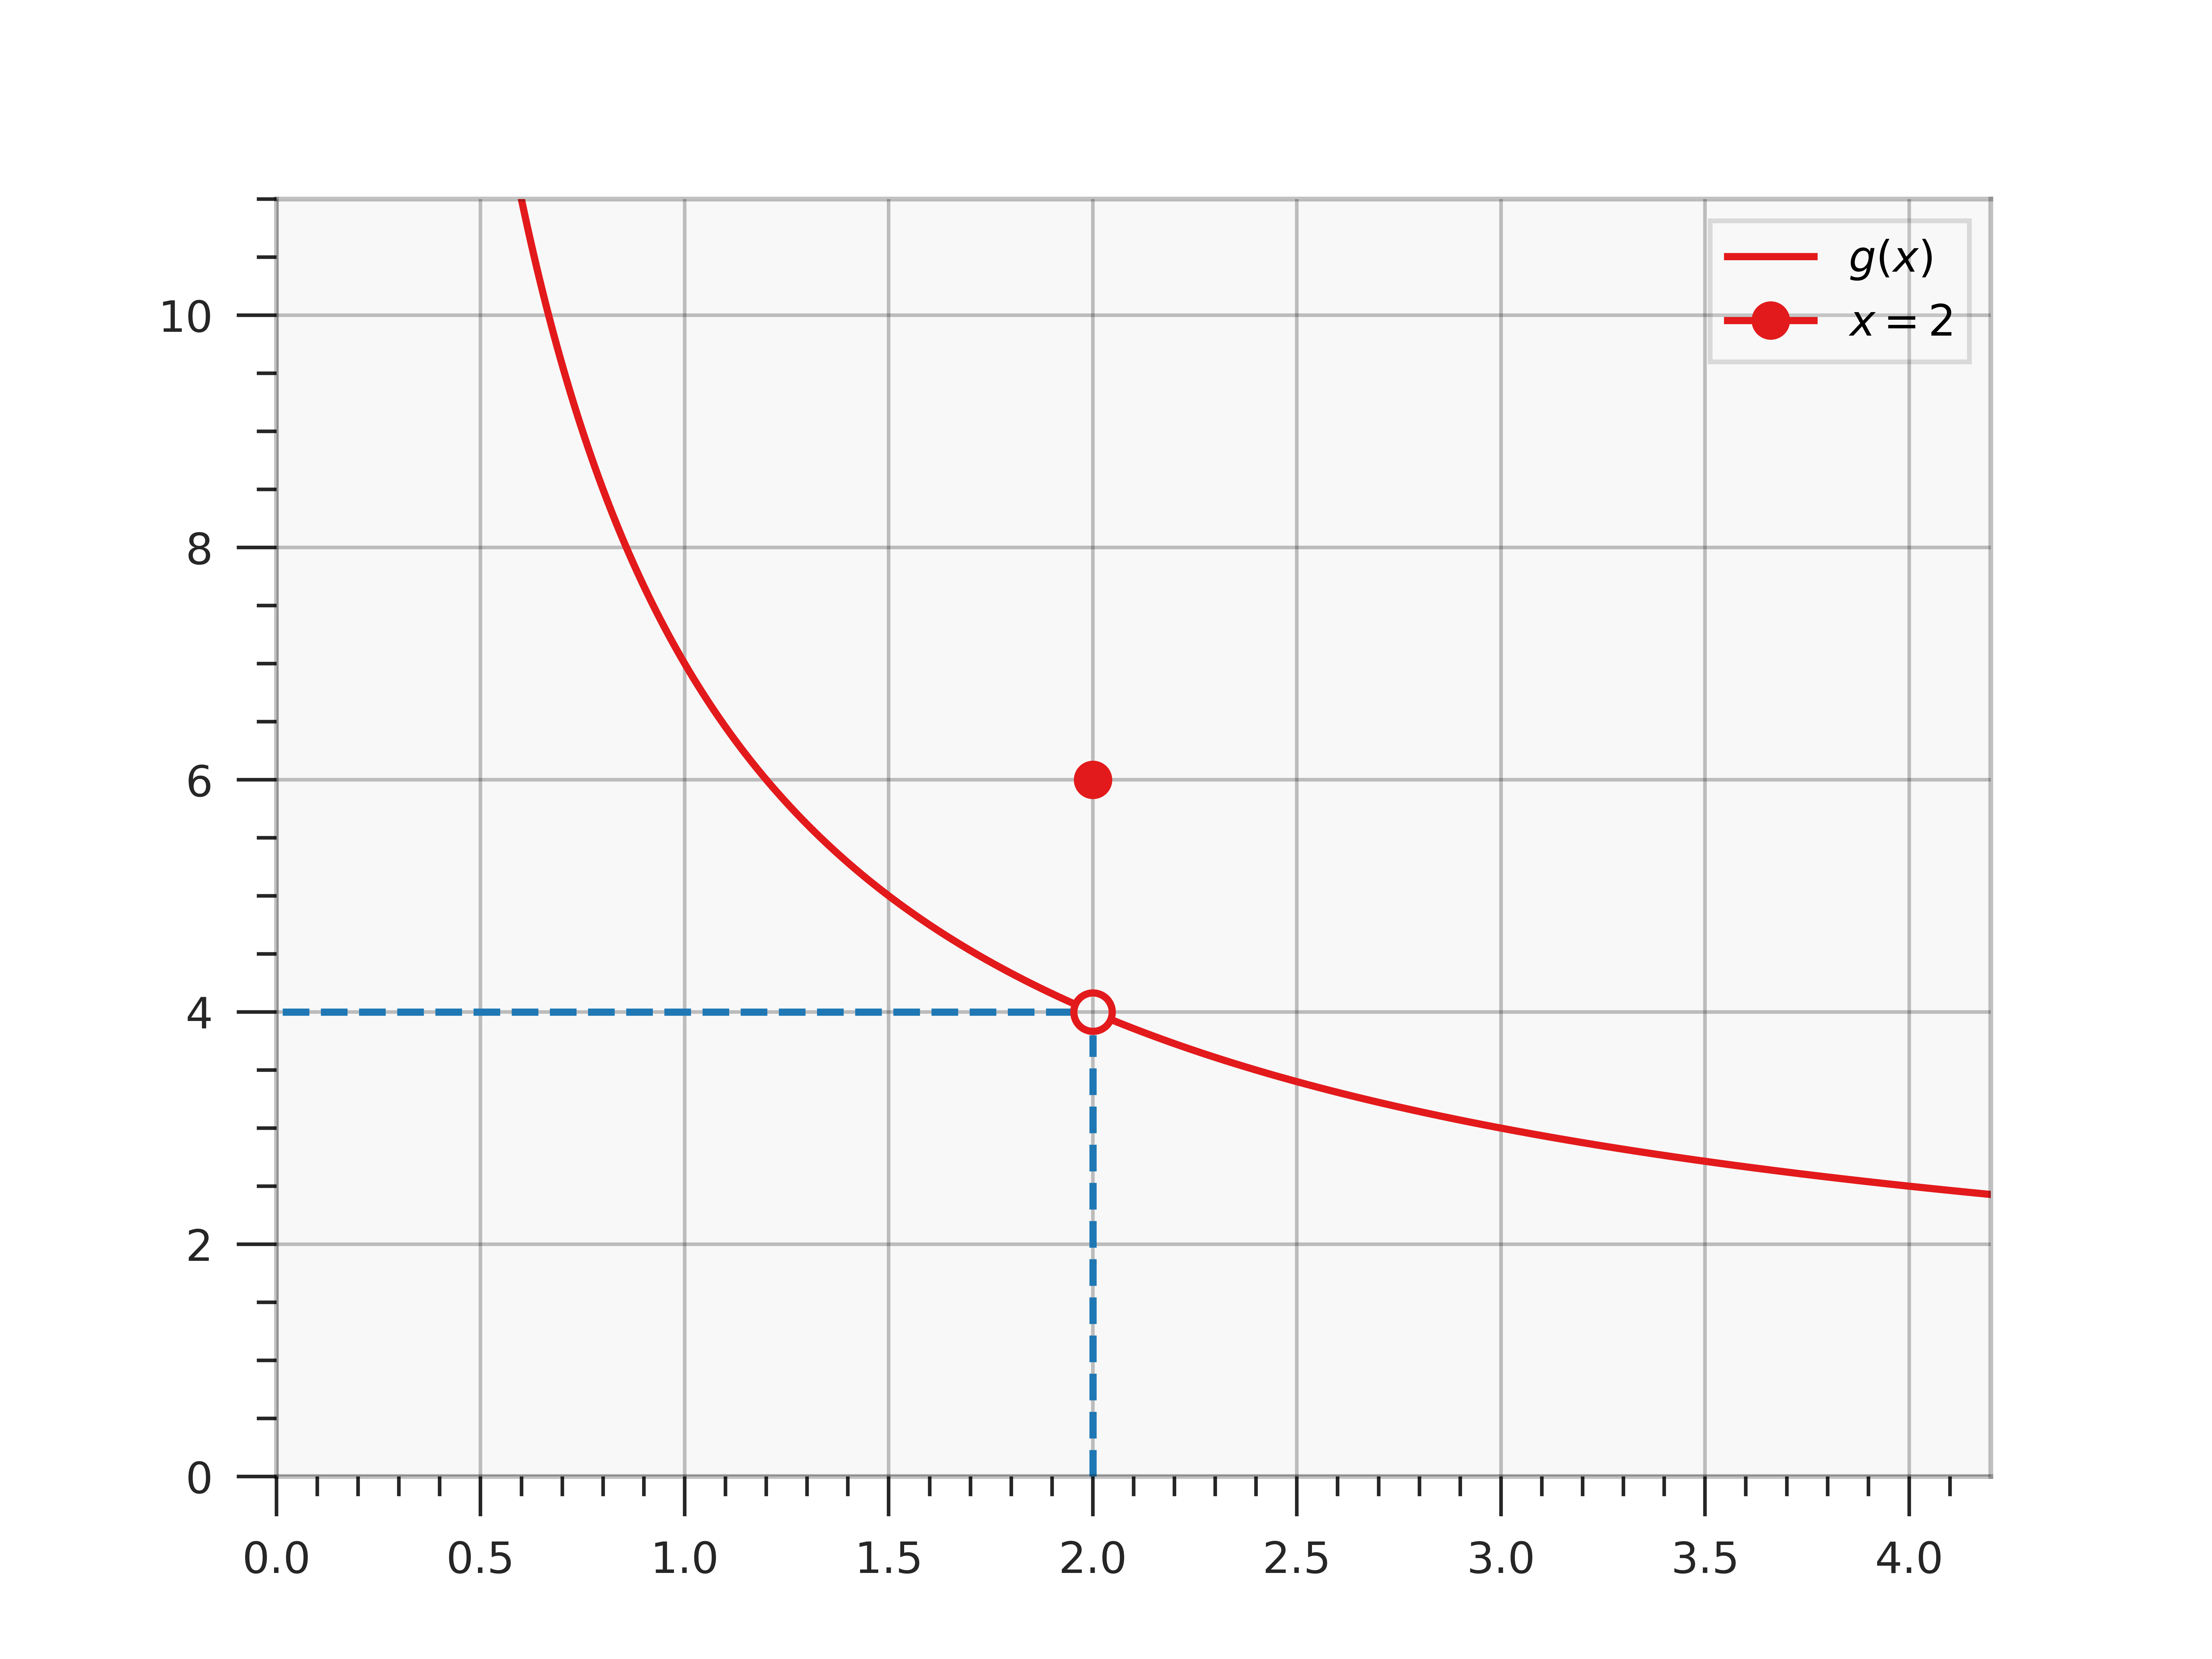
\includegraphics[width=12.5cm, keepaspectratio]{limits_2.png}
    \caption{Limits of Piecewise Functions}
    \label{fig:fig2}
\end{figure}

As we move towards $x=2$ from both sides, it is still approaching 4.
While there is now a dot at $(2, 6)$, this is not what the function approaches so our limit remains as 4 as that is what is going on around the function.
This idea that limits are not concerned with the value at the target point is very important and we should keep it in mind.
Let's look at another problem.

\begin{problem}
Estimate the value of:
\begin{equation*}
    \lim_{\theta\to0} \frac{1-\cos(\theta)}{\theta} \label{eq:4}
\end{equation*}
\end{problem}

The variable we are dealing with in this situation is $\theta$ and not something like $x$ or $t$ but it makes no difference to how we tackle the problem.
Also note that we cannot evaluate the function at $\theta=0$ as we would be dividing by 0.
The function not existing at $\theta=0$ does not mean that the limit as $\theta$ approaches 0 does not exist as well.
Below is a table of values for it.

\begin{table}[h]
    \renewcommand{\arraystretch}{1.5}
    \centering
    \begin{tabular}{>{\centering\arraybackslash}m{1.5cm}|>{\centering\arraybackslash}m{2.5cm}|>{\centering\arraybackslash}m{1.5cm}|>{\centering\arraybackslash}m{2.5cm}}
        $\theta$ & $f(\theta)$   & $\theta$ & $f(\theta)$           \\ \hline
        $1$      & $0.45969769	$ & $-1$     & $-0.45969769        $ \\
        $0.1$    & $0.04995835$  & $-0.1$   & $-0.04995835$         \\
        $0.01$   & $0.00499996$  & $-0.01$  & $-0.00499996$         \\
        $0.001$  & $0.00049999$  & $-0.001$ & $-0.00049999$
    \end{tabular}
\end{table}

Since we see that the function appears to be approaching $0$ as $\theta$ approaches 0 from both sides, we can estimate the limit to be 0.
This turns out to be the actual value of the limit, so the solution to Problem~\eqref{eq:4} is the following.

\begin{equation}
    \lim_{\theta\to0} \frac{1-\cos(\theta)}{\theta} = 0
\end{equation}

Once again, while the value of the function did not exist at our target point, we were able to estimate the value of the limit for it.
Sometimes, it may be the case that the value of a function will be the same as its limit, but we would go by finding this limit just as we have with the previous examples; we create a table of values or sketch a graph of the function to notice what value the function approaches, if any.
Let's look at another example that is slightly different.

\begin{problem}
Estimate the value of:
\begin{equation*}
    \lim_{t\to0} \cos\left(\frac{\pi}{t}\right) \label{eq:5}
\end{equation*}
\end{problem}

We are obviously not able to evaluate the function directly at $t=0$.
Let us create a table of values to see the behaviour of the function as $t$ goes to 0.

\begin{table}[H]
    \renewcommand{\arraystretch}{1.5}
    \centering
    \begin{tabular}{>{\centering\arraybackslash}m{1.5cm}|>{\centering\arraybackslash}m{2.5cm}|>{\centering\arraybackslash}m{1.5cm}|>{\centering\arraybackslash}m{2.5cm}}
        $t$     & $f(t)$ & $t$      & $f(t)$       \\ \hline
        $1$     & $-1	$  & $-1$     & $-1        $ \\
        $0.1$   & $1$    & $-0.1$   & $1$          \\
        $0.01$  & $1$    & $-0.01$  & $1$          \\
        $0.001$ & $1$    & $-0.001$ & $1$
    \end{tabular}
\end{table}

From this, we might want to estimate the limit to be 1.
However, if we did this, we would be incorrect; consider the following evaluations of the function to see why.

\begin{equation*}
    f\left(\frac{1}{2001}\right) = -1 \qquad f\left(\frac{2}{2001}\right) = 0 \qquad f\left(\frac{4}{4001}\right) = \frac{\sqrt{2}}{2}
\end{equation*}

All of these evaluations use values of $t$ less than 0.001.
Yet, we get completely different numbers.
Definition~\eqref{eq:1} requires a function to be as close, or get closer, to a value as our variable gets closer to its target point.
At the very least, that means that $t=0.001$ is certainly not close enough to 0 for $f(t)$ to remain close to some value.
To see what is going on with our function, it would help to sketch a graph for it.

\begin{figure}[H]
    \centering
    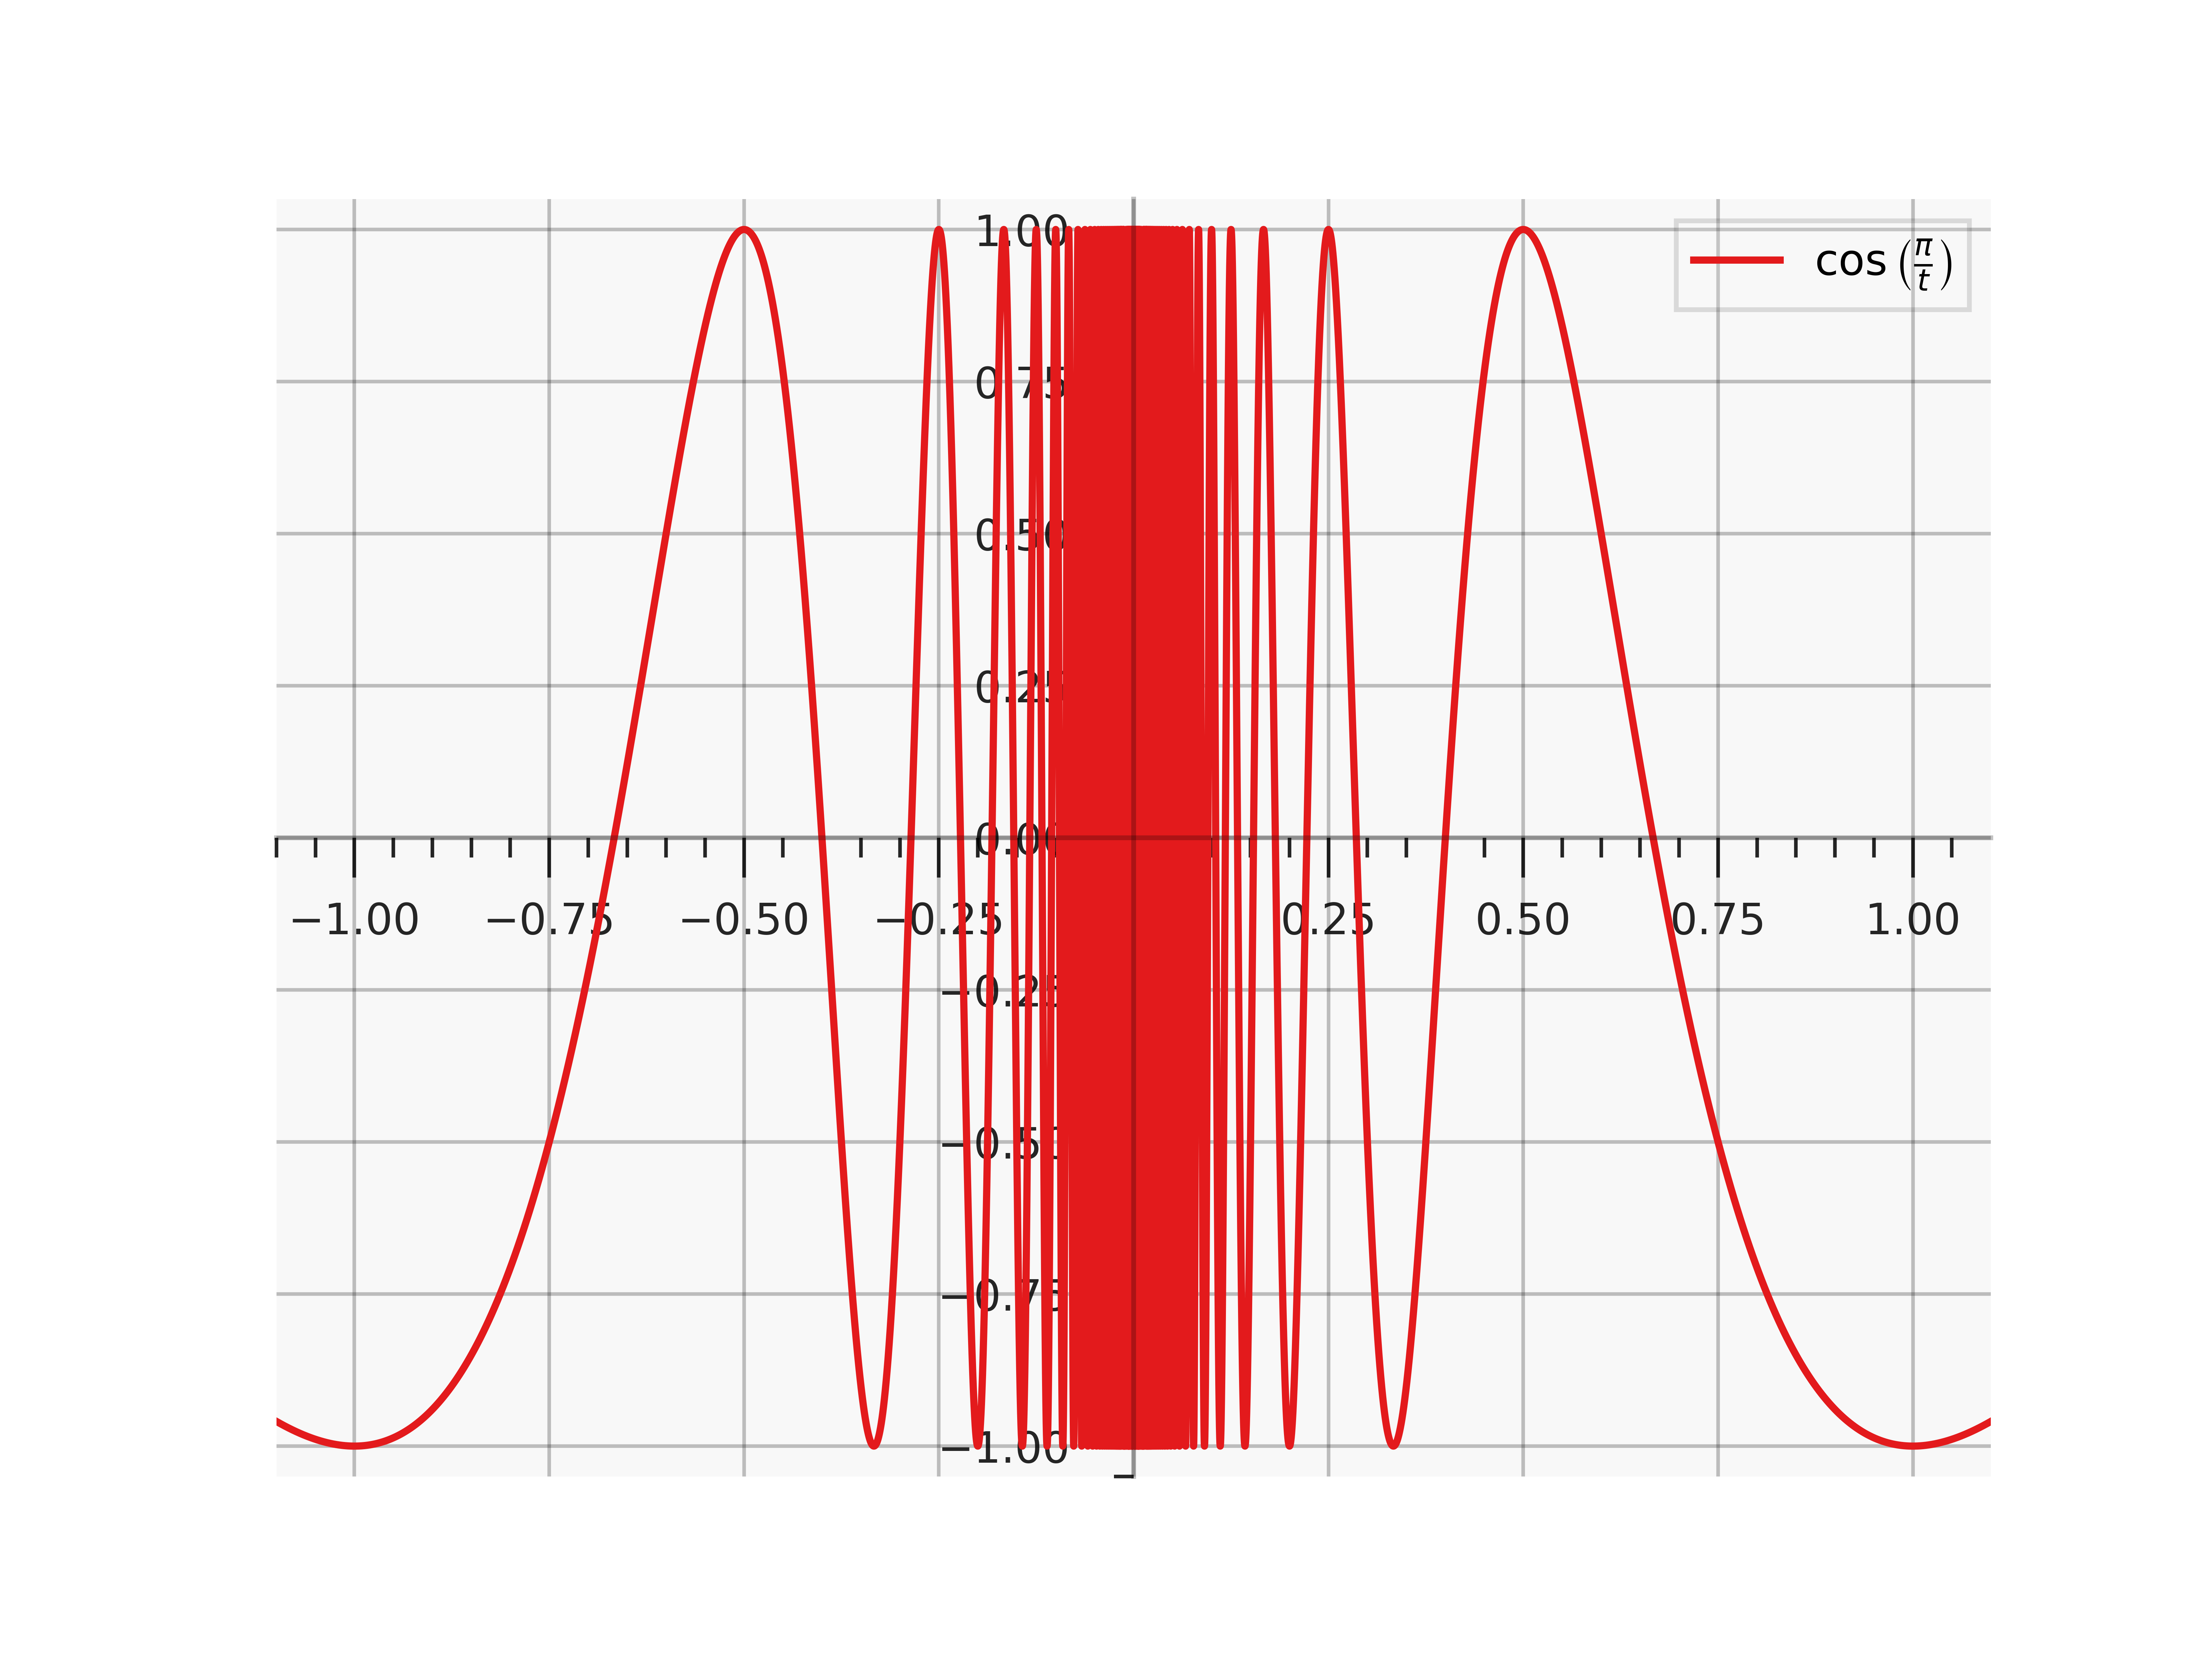
\includegraphics[width=12.5cm, keepaspectratio]{limits_3.png}
    \caption{Limits of Oscillatory Functions}
    \label{fig:fig3}
\end{figure}

From this graph, we can see that as we approach, $t=0$, the function oscillates faster and faster.
From our definition of a limit, the function must settle down to some value as we approach our target variable.
Due to the fact that the function wildly oscillates as we approach our target value, there is no value of $t$ that will be close enough to 0 such that all values of $t$ even closer to 0 will make $f(t)$ as close to any number $L$ as we want; we would be able to choose some difference between $f(t)$ and some number $L$, such that no matter how close our chosen value of $t$ was to 0, there would be some number closer which would not make $f(t)$ as close to $L$ as we want.
Therefore, as the function does not settle to any one value as we approach $t=0$, we can answer Problem~\eqref{eq:5} by saying that the limit does not exist.

Problem~\eqref{eq:5} shows the issues with using a table of values to estimate limits.
The value we used in our table were perfectly fine and were the same as we did in the problem before that which gave us the correct idea of what the function was approaching.
Using a table of values will always mean that there is a chance that we are not choosing the right values and will incorrectly guess the limit.
That is something very important to keep in mind when using them for limits; the problem is major enough that we will never use a table of values to estimate after this section.

The previous problem has also shown us that a limit may sometimes not exist at all if the function is not approaching any value.
Let's look at one more example.

\begin{problem}
Estimate the value of:
\begin{equation*}
    \lim_{x \to 0} H(t), \quad H(t) =
    \begin{cases}
        0 & \text{if } t < 0    \\
        1 & \text{if } t \geq 0
    \end{cases} \label{eq:6}
\end{equation*}
\end{problem}

$H(t)$ is often called the Heaviside step function.
While we could create a table of values, making a graph for this function is just as simple.

\begin{figure}[H]
    \centering
    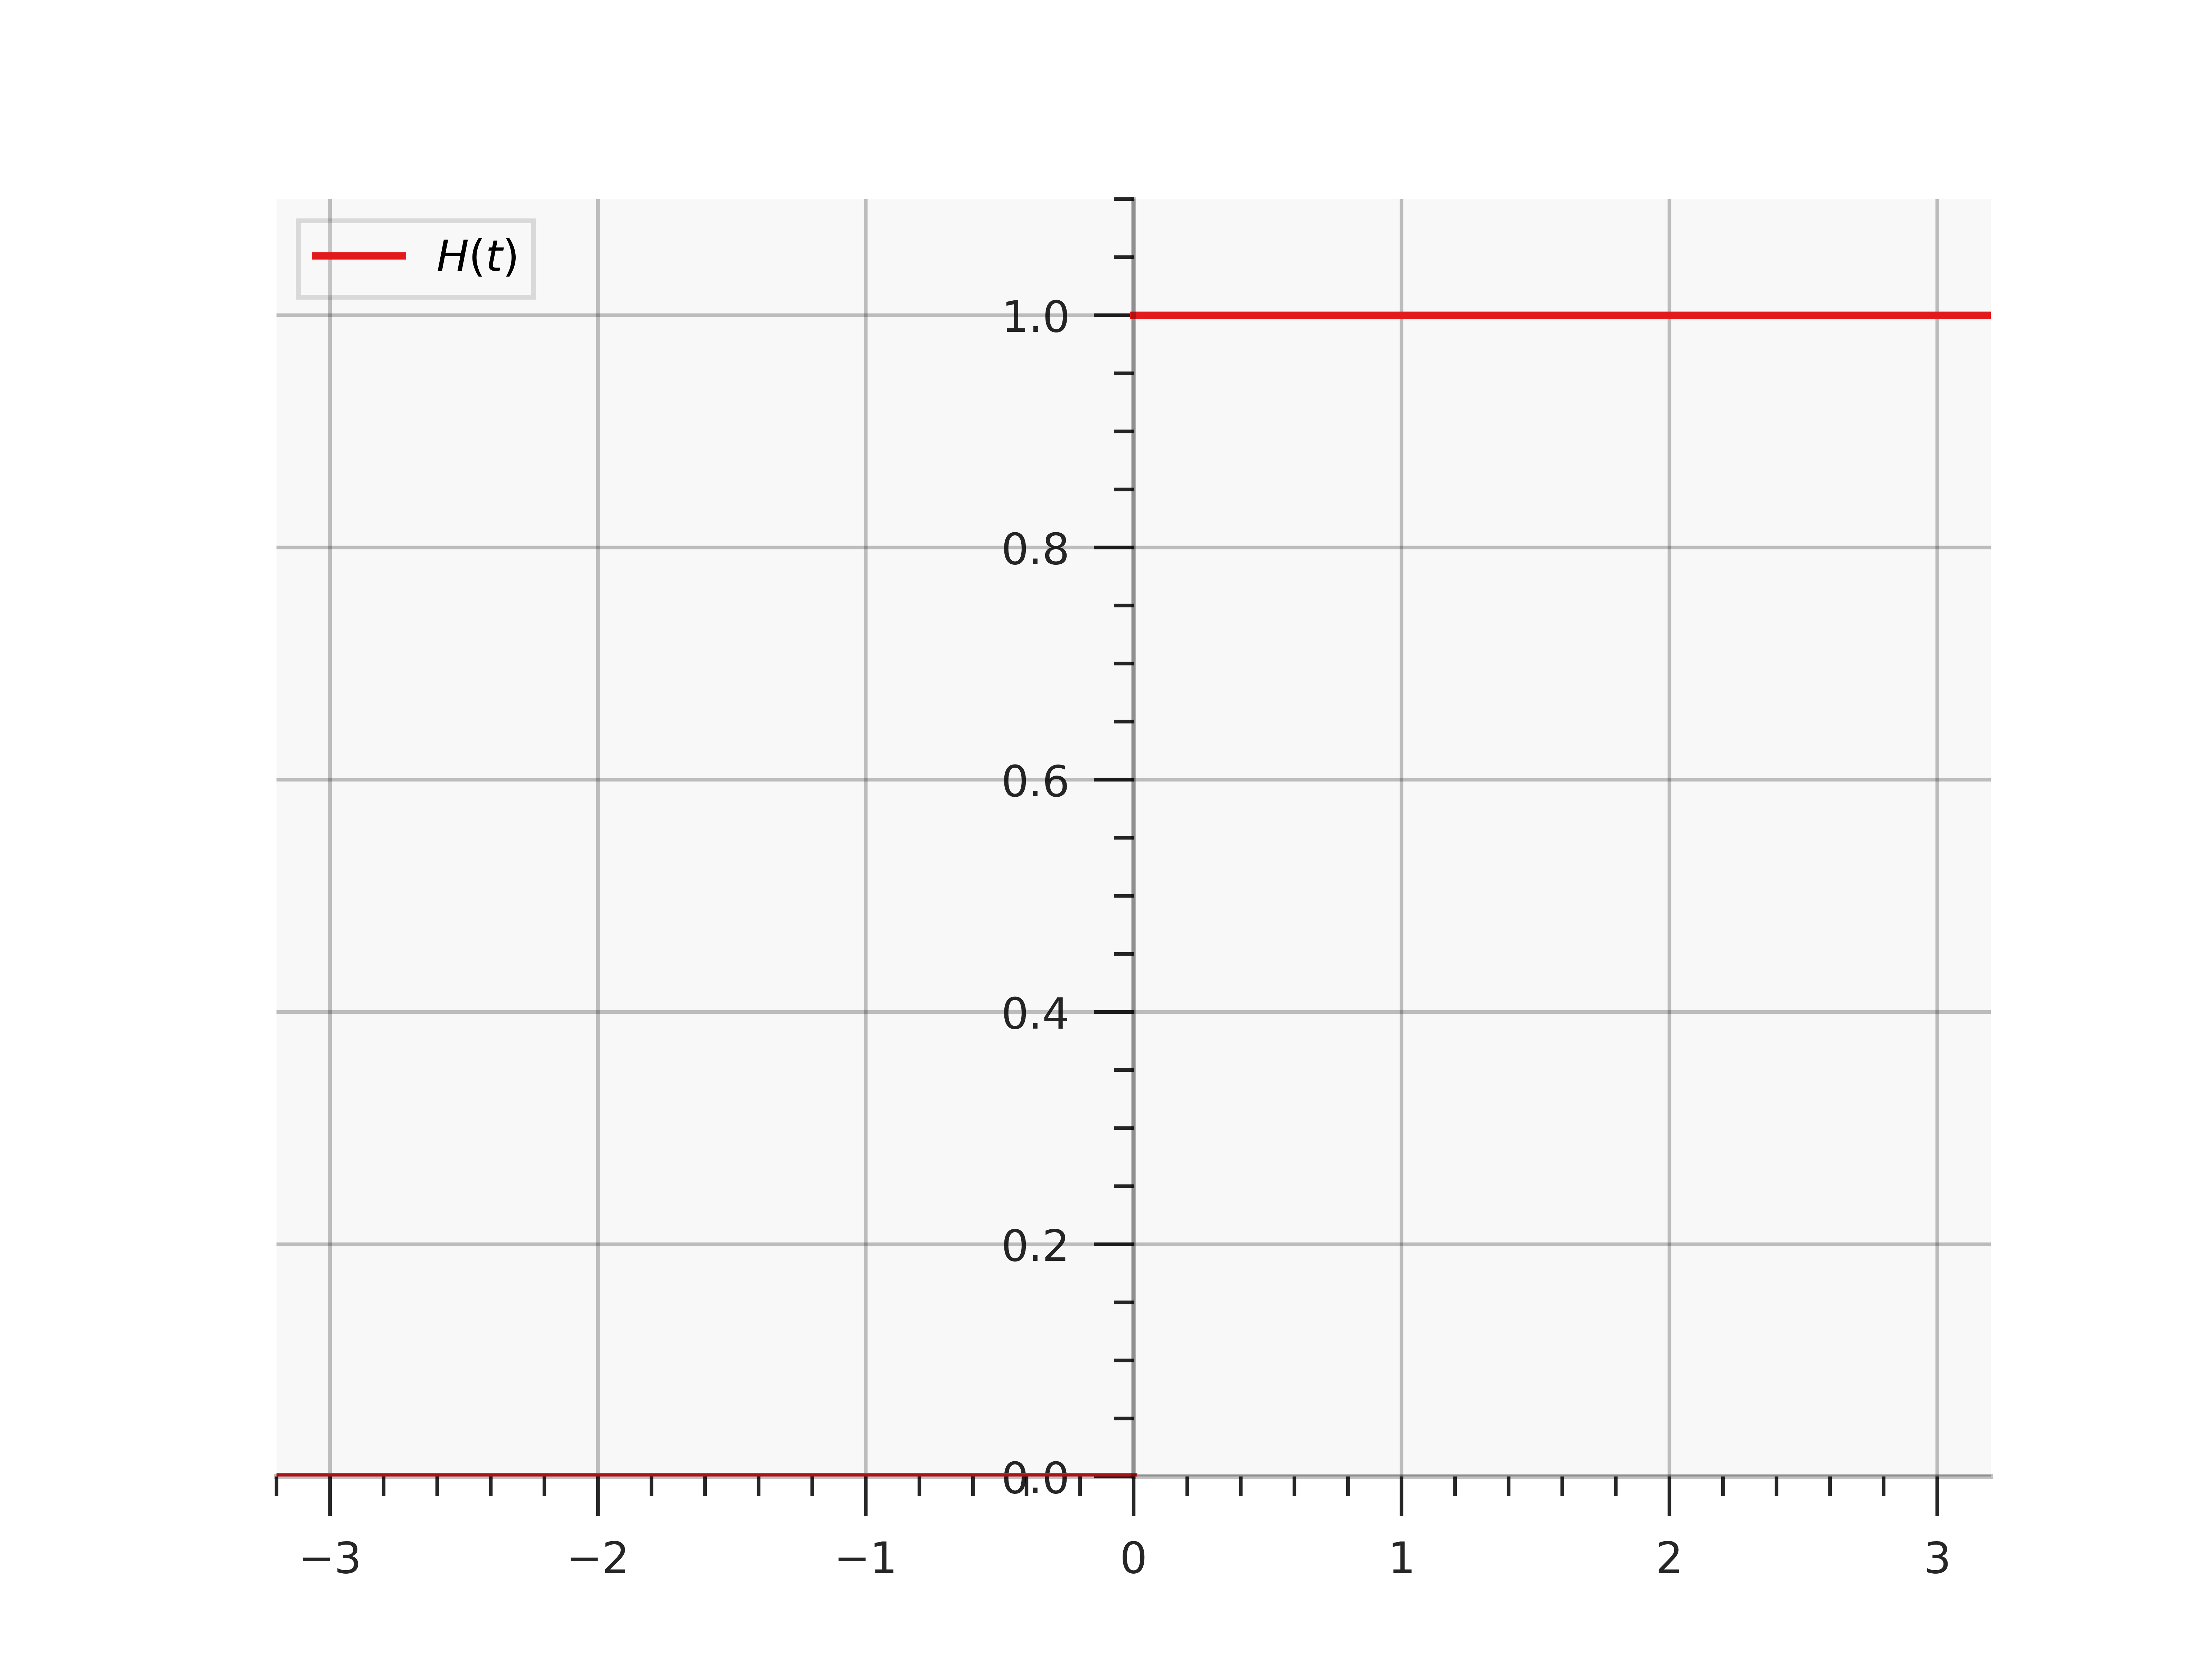
\includegraphics[width=12.5cm, keepaspectratio]{limits_4.png}
    \caption{Heaviside Step Function}
    \label{fig:fig4}
\end{figure}

If we approach $t=0$ from the right, we can see it goes to 1; it does have 1 as its value for all nonnegative numbers.
If we approach $t=0$ from the left, the function approaches 0 as its value as it stays at 0 until it gets to $t=0$.
Since the function must approach the same value from both sides of our point, the limit does not exist for Problem~\eqref{eq:6}.

This is slightly different from the previous problem.
While in both instances, the limit does not exist, that happens for two different reasons.
One is because the function oscillates so it does not settle at any one value while we approach our target point; in the other problem, the function approaches two different values from the left and right.
We will discuss the latter case further in the next section.

The first three problems which we have looked at have shown us that the limit of a function at some point is not necessarily the value of the function at that point.
It may be the case that a limit exists even when the function doesn't if it still approaches some value.
Conversely, it may be the case that the limit of a function does not exist even when the function is defined at that point.
This may because the the function does not settle towards any single value or that it approaches different values from each side.

We should not assume at this point that the limit and the value of a function at some point will be the same, or that one of them existing means that the other will.
Most of the time, we will deal with limits that do exist; we should not thus assume that a limit will exist in general.
We have also seen the problems of using tables of values and how they can lead us to believe a completely wrong conclusion; tables of values are not reliable and should be the last way we consider to find a limit.

While we have seen using graphs for limits to be more reliable, there are some setbacks to it.
To be able to use a graph, we must need to actaully create it which may not be so easy to do for some functions.
Additionally, graphs are only really useful if $f(x)$ is approaching some integer.
If it isn't, then it is practically impossible to guess the $y$ value that it is approaching from the graph.
How do you guess that $f(x)$ approaches 7.135 from a graph?
You can't.

Usually, we do want to know what the limit is exactly and not just estimate it, so neither tables of values nor graphs are the best to use.
The reason we have used them in this section is because they help to show what limits actually represent and to show some methods which are not as good so we do not use them regularly.
We will discuss how to properly evaluate limits in the next few sections, but there are some important things that must be considered prior.

\end{document}